% Documentation of template:
% https://mirror.koddos.net/CTAN/macros/latex/contrib/beamer-contrib/themes/metropolis/doc/metropolistheme.pdf

\documentclass{beamer}
\usetheme[progressbar=head, numbering=fraction, background=light]{metropolis}% Use metropolis theme
\usepackage{preamble}

\title{$p$-adic Numbers and Newton polygons}
\date{\today}
\author{Yoav Eshel, Anh Van Giang}
\institute{Vrije Universiteit Amsterdam}


\begin{document}
    \maketitle
    \begin{frame}{Preliminaries}
        \begin{itemize}
            \item Cauchy sequence
            \item Rings, Fields
            \item Algebraic Closure
        \end{itemize}
    \end{frame}
    \section{Introduction}
    \begin{frame}{Hensel's Analogy}
        $\Q$ is the field of fractions of $\Z$, $\C(X)$ is the field of fractions of $\C[X]$\pause
        
        Any element in $\Z$ has a unique factorization in primes $p_i$, any polynomial $\C[X]$ has a unique factorization in the primes $(X-\alpha)$
    \end{frame}
    \begin{frame}{$p$-adic integers}
        Any polynomial $P(X)\in\C[X]$ can be expanded as $P(X)=\sum_{i=0}^n a_i(X-\alpha)^i$.
        Any Integer $a\in\Z$ can be expanded in base $p$\pause
        
        For example
        $$72=0+0\cdot 3+2\cdot3^2+2\cdot 3^3$$
    \end{frame}
    \begin{frame}{$p$-adic numbers}
        Every rational function $f(X)\in\C(X)$ has a Laurent series $f(x)=\sum_{i\geq n} a_i(X-\alpha)^i$.
        
        We can do the same thing with rational numbers: 
        
        Let $p=3, a=24, b=17$. Formally dividing
        $$\frac{a}{b}=\frac{24}{17}=\frac{2p+1p^2}{2+2p+p^2}=p+p^3+2p^5+p^7+p^8+2p^9+\cdots$$\pause
        
        (You can verify the above calculation by multiplying the expansions of $\frac{a}{b}$ and $b$)
    \end{frame}
    % \begin{frame}{$p$-adic numbers}
    %     Conclusion: every rational number can formally be written as a finite tailed series in powers of $p$.
        
    %     The field of all finite tailed series in $p$ is denoted $\Qp$.
    % \end{frame}
    
    \section{$p$-adic Numbers}
    \begin{frame}{Introducing a new metric}
    \begin{definition}
        Let $p$ a fixed prime, define the $p$-adic valuation of $a \in \Z$, $\valp{(a)}$, as the highest exponent $m$ such that $p^m$ divides $a$ with $\valp{(0)} = \infty$.
    \end{definition}
    For example, $\val5{(15)} = 1$ and $\val3{(54)} = 3$.\\
    This valuation map behaves like the logarithm:
     \[ \valp{(a_1 a_2)} = \valp{(a_1)} + \valp{(a_2)}, \ \valp{(a_1/a_2)} = \valp{(a_1)} - \valp{(a_2)}. \]
    \end{frame}
    
    \begin{frame}{Introducing a new metric}
        
     \begin{definition}
         Define the $p$-adic absolute value $\absp{\cdot}$ on $\Q$ as:
         \begin{equation*}
            \absp{x} = 
            \begin{cases}
               p^{-\valp(x)} & \text{if}\ x \neq 0\\
                0, & \text{if}\ x = 0.
            \end{cases}
    \end{equation*}
     \end{definition}
     
     This is a non-Archimedean norm i.e. $\absp{x + y} \leq \max(\absp{x}, \absp{y})$.\\
     The usual and familiar norm on $\Q$ is Archimedean.\\
     This norm induces a non-Archimedean metric in $\Q$.
    \end{frame}
    
    \begin{frame}{Introducing a new metric}
    Fun facts about a non-Archimedean metric in $\Q$:\\
    \indent $(i)$ Every point in a disc is the center.\\
    \indent $(ii)$ Every triangle is an isolesces triangle.
    \end{frame}
    
    \begin{frame}{Constructing $\Q_p$}
    
    Why ?
        
    \end{frame}
    
    \begin{frame}{Constructing $\Q_p$}
    
    Because $\Q$ is not complete with respect to $\abs{\cdot}_{\infty}$ or $\absp{\cdot}$.\\
        
    \end{frame}
    
    \begin{frame}{Constructing $\Q_p$}
    
    Not all Cauchy sequences converge in $\Q$. 
        
    \end{frame}
    
    \begin{frame}{Constructing $\Q_p$}
    \begin{theorem}
        (Ostrowski) Every non-trivial norm on $\Q$ is equivalent to the $p$-adic norm $\absp{\cdot}$ or the Euclidean norm $\abs{\cdot}_{\infty}$.
    \end{theorem}
        
    \end{frame}
    
        
    
    \begin{frame}{Constructing $\Q_p$}
    
    For the standard norm, take the Cauchy sequence 
    \[a_n = \frac{f_{n+1}}{f_n} \ \text{where $\langle f_n \rangle$ is the Fibonacci sequence} \]
    which converges to the golden ratio $(1+\sqrt{5})/2$ not in $\Q$ because it is irrational so $\Q$ is not complete under $\abs{\cdot}_{\infty}$.\\
    \end{frame}
    
    \begin{frame}{Constructing $\Q_p$}
    
    Can we actually construct $\Q_p$ ? Is it unique ?
        
    \end{frame}
    
    \begin{frame}{Constructing $\Q_p$}
        \begin{theorem}
            Let $(K, \abs{\cdot})$ be a normed field. Then there exists a complete field $K^'$ with a norm $\abs{\cdot}^{'}$ that extend $K$. This completion is unique up to isomorphism. If $\abs{\cdot}$ is non-Archimedean then so is $\abs{\cdot}^{'}$. 
        \end{theorem}
        $\Qp$ can be constructed by letting it be the set of equivalence classes then $\Q$ is the subfield of $\Q_p$ consisting of constant Cauchy sequences.
        \end{frame}
    
    \begin{frame}{Hensel's lemma}
    
    \begin{definition}
        For a fixed prime $p$, a $p$-adic number is a series of the form 
\[\sum_{i=k}^{\infty} a_i p^i \ \text{where }a_i \in \{0,1,...,p - 1\}. \]
If $\sum_{i=k}^{\infty} a_i p^i = x \in \Qp$ then the series is called a $p$-adic expansion of $x$.
    \end{definition}
    
    \end{frame}
    
    \begin{frame}{Hensel's Lemma}
    
    If $k \geq 0 $ then the $p$-adic number is called a $p$-adic integer.\\
    The set of all $p$-adic integer forms a ring $\Z_p$.
        
    \end{frame}
    
    \begin{frame}{Hensel's lemma}
    
    \begin{theorem} Let $F(X) = c_0 + c_1 X + c_2 X^2 + ... + c_n X^n$ be a polynomial whose coefficients are in $\Z_p$. Suppose that there exists a $p$-adic integer $a_0 \in \Z_p$ such that 
\[F(a_0) \equiv 0 \ \text{mod $p$} \]
and 
\[F^{'}(a_0) \not\equiv 0 \  \text{(mod $p$)}\]
where $F^{'}$ is the derivative of $F$. Then there exists a unique $p$-adic integer $\alpha \in \Z_p$ such that $\alpha \equiv a_0 \mod p$ and $F(\alpha) = 0$.
    \end{theorem}
        
    \end{frame}
    
    \begin{frame}{Hensel's Lemma}
    Proof:
        Similar to the approximation technique used in Newton's method.
    \end{frame}
    
    \begin{frame}{Hensel's Lemma}
    Construct a sequence of integers $a_1,a_2,a_3,...$ with $a_n = a_{n-1} + b^n p^n$.\\
    \end{frame}
    
    \begin{frame}{Hensel's Lemma}
    Construct a sequence of integers $a_1,a_2,a_3,...$ with $a_n = a_{n-1} + b^n p^n$.\\
    \[b_n p^n \equiv \frac{-\alpha^{'}}{F^{'}(a_{n-1})} \equiv \frac{F(a_{n-1})}{F^{'}(a_{n-1})} \ \text{mod $p^{n+1}$}. \]
    \end{frame}
    
    \begin{frame}{Hensel's Lemma}
    Example: 
    Solve $F(X) = X^3 - 2$ in $\Z_5$.\\
    Initial approximation $a_0 = 3$.\\
    Solution: $3 + 2 \cdot 5^2 + 2 \cdot 5^3 + ...$
        
    \end{frame}
        

    
    \section{Completions and Algebraic Closures}
    \begin{frame}{Absolute Value Extends Uniquely}
        \begin{theorem}
            Let $K$ be a complete field with respect to a non-archimedean absolute value $\abs{\cdot}$ and $L/K$ algebraic. Then there is a unique extension $\abs{\cdot}'$ of $\abs{\cdot}$ to $L$. If $[L:K]=n$, then the extension is given by
            $$\abs{\alpha}'=\sqrt[n]{\abs{N_{L/K}(\alpha)}},\quad \alpha\in L$$
        \end{theorem}
        \begin{proof}
            \cite[p. 131]{jurgen_99}
        \end{proof}
    \end{frame}
    % \begin{frame}{Absolute Value Extends Uniquely}
    %     It is easy to verify that the extension agrees with the absolute value on $K$:
    %     \[\abs{\alpha}'=\sqrt[n]{\abs{N_{L/K}(\alpha)}}=\sqrt[n]{\abs{\alpha^n}}=\abs{\alpha},\quad \alpha\in K\]
    %     and that 
    %     $$\abs{\alpha}'=0\iff\alpha=0,$$ $$\abs{\alpha\beta}'=\abs{\alpha}'\abs{\beta}'.$$
    % \end{frame}
    % \begin{frame}{Absolute Value Extends Uniquely}
    %     It is harder to check that $\abs{\alpha+\beta}\leq\max\{\abs{\alpha},\abs{\beta}\}$ and to verify uniqueness. 
    % \end{frame}
    
    \begin{frame}{$\overline{\Qp}$ is not complete}
        \pause
        \begin{itemize}
            \item The standard procedure is to construct a Cauchy sequence the does not have a limit in $\overline{\Qp}$.\pause
            \item Instead, we show that in a complete metric space the union of closed sets with empty interiors has an empty interior as well (\textit{Baire Category Theorem}, \cite[p. 296]{munkres_2014}).\pause
            \item Any finite dimensional subspace of a normed vector space over a complete field is closed.\pause
            \item Proper subspaces of normed vector spaces have an empty interior.\pause
            \item As $\overline{\Qp}/\Qp$ has a countable degree (\cite[p. 54]{lang_1986}), it follows that $\overline{\Qp}$ is not complete.
        \end{itemize}
    \end{frame}
    
    \begin{frame}{The completion of an algebraic closure is algebraically closed}
        \begin{theorem}
            Let $K$ be a complete field with a non-archimdean and non-trivial absolute value $\abs{\cdot}$. Then the completion $L$ of $\overline{K}$ is algebraically closed.
        \end{theorem}\pause
        \begin{proof}
            Any root of a polynomial over $L$ will be the limit of a sequence in $\overline{K}$.
        \end{proof}
    \end{frame}
    
    \begin{frame}{Did we choose the hard way on purpose?}
        Why not take the algebraic closure $\overline{\Q}$ of $\Q$ and then complete it with respect to the $p$-adic norm to get $\Cp$?\pause
        
        Because there a lot more absolute values on $\overline{\Q}$ than there are on $\Q$.
    \end{frame}
    \section{Analysis in $\Cp$}
    \begin{frame}{Some notable results}
        \begin{itemize}
            \item If $a_n\to a\neq 0$, then $\absp{a_n}=\absp{a}$ for sufficiently large $n$\pause
            \item A series $\sum_{n} a_n$ in $\Cp$ converges \textbf{if and only if} $\absp{a_n}\to 0$\pause
            \item A sequence $\langle a_n\rangle$ in $\Cp$ is Cauchy \textbf{if and only if} $\absp{a_n-a_{n+1}}\to 0$\pause
        \end{itemize}
    \end{frame}
    
    \begin{frame}{Newton polygons}
        Let $f(X)=1+a_1X+\cdots+a_nX^n\in\Cp[X]$,
    
        The Newton polygon of $f(X)$ is the lower convex hull of 
        $$\{(i, v_p(a_i))\}$$
        ignoring the points $a_i=0$.
    \end{frame}
    \begin{frame}{Newton polygons}
        Let $p=5$ and $f(X)=1+5X+\frac15X^2+35X^3+25X^5+625X^6$\pause
        \begin{figure}
            \centering
            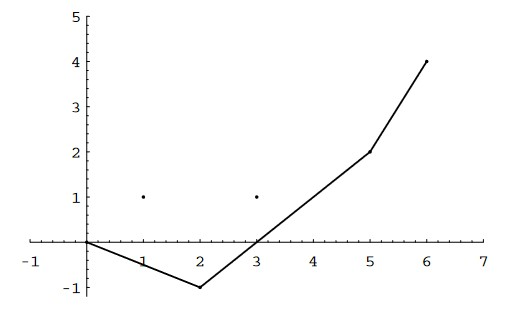
\includegraphics[width=8cm]{img/newtonpolygon.jpg}
            \caption{Newton polygon for $f(X)$}
            \label{fig:newtonpolygon}
        \end{figure}
    \end{frame}
    \begin{frame}{Newton polygons}
        \begin{theorem}
            Let $f(X)=1+a_1X+\cdots+a_nX^n\in\Cp[X]$, let $m_1\leq m_2\leq\cdots\leq m_r$ be the slopes of its Newton polygon and $i_1,i_2,\dots,i_r$ the corresponding lengths. Then $f$ has exactly $i_k$ roots (counting multiplicity) of absolute value $p^{m_k}$.
        \end{theorem}
        \pause
        
    \end{frame}
    \begin{frame}{Newton polygons for power series}
        \begin{theorem}
            Let $m$ be the supremum of the slopes of a (formal) power series $f(X)\in\Cp[[X]]$. Then the radius of converges of $f$ is $p^m$ (or $+\infty$ if $m=\infty$).
        \end{theorem}
        \pause
        As for any $\absp{x}=p^{m'}<p^m$, the point $(i,\valp{(a_i)})$ will lie above $(i, m'i)$ for $i$ sufficiently large. So $\valp{(a_i)}\to\infty$ and $f(x)$ converges.
    \end{frame}
    \section{Conclusion}

    
    \begin{frame}[standout]
        Thank you! Questions?
    \end{frame}
    
    \section{References}
    \bibliographystyle{unsrt}
    \bibliography{references}
\end{document}